\chapter{Gaussian Mixture Models}
\section{Theory}

Gaussian Mixture Models (GMM) is a way of finding and describing sub-populations in clusters of data points. 
It is done by fitting a specified number of Gaussian distributions to a population of data points.
Each distribution is a component of the model. 
The individual data points are then arranged into clusters based on which model component is most likely given the observed data point.

In this context the data points are features in a multidimensional feature space. Hence the distributions used for the GMM is multivariate Gaussians.

The clustering on basis of likelihood makes GMMs more robust than e.g. K-means, where data points are clustered similarly, but simply on the basis of Euclidean distance to the center of a model. 
This is because treating the components like Gaussians with means and variances instead spheres with uniform probability, gives a more nuanced picture of the strength of a data point’s relationship to a model component. 
It also gives rise to the notion of soft relations to clusters or data points related to more than one cluster.

When fitting the GMM the goal is to maximize the overall likelihood of the model for the entire population.
Firstly it is necessary to determine the number of distribution components the data should be fitted to. 
The number of distributions needed in a GMM greatly depends on the nature and origin(s)
of data.
This, however, does not mean that if a mixture model fits data well with a specific amount of distributions, then this is the actual number of sub-populations, or sources if you will.
Multiple sub-populations could be grouped together, or likewise sub-populations could be split, due to under/over-fitting.
For this reason experimentation is necessary to establish the optimal number of distributions needed to model data.

\fxnote{ What we did for this project (Måske under metode)}

% Afsnit om EM-algoritmen til GMM
\fxnote{Ref}
\subsection{The EM Algorithm}
The distributions of the mixture model are fitted to data by iteratively employing Expectation Maximization (EM).
This is done by either selecting an arbitrary guess of the means and variances of the model as a starting point or initializing the means with a few iterations of K-means, and setting the covariance matrices to the identity matrix. 
The latter is often used because even though GMM generally is more precise than K-means, it is also much more computationally heavy.
Therefore by initializing with K-means, a relatively light algorithm, the EM will converge on a good model faster.

A visual example of this convergence can be shown by applying GMM to dataset of eruption time vs. waiting time of the Old Faithful geyser in Yellowstone National Park, WY, USA.
The data has been normalized for simplicity. 
\\

\begin{figure}[H]
\centering
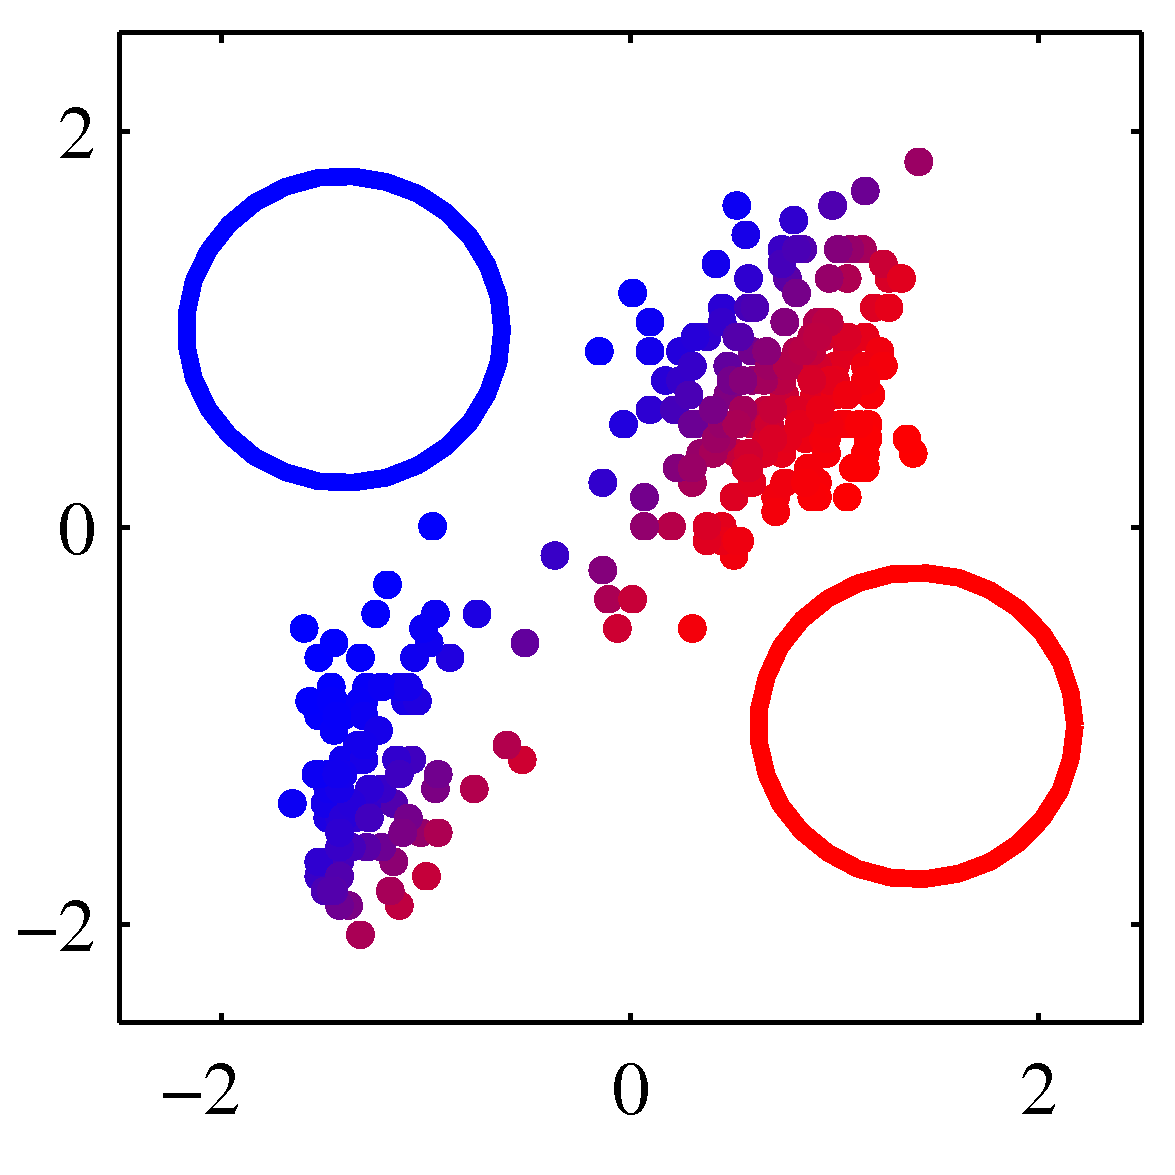
\includegraphics[width=0.25\textwidth]{GMM1}
\caption{Old Faithful data. GMM stared at an abitrary point}
\label{fig:GMM1}
\end{figure}

In Figure \ref{fig:GMM1} above the EM has just started from an arbitrary starting point.
Data shows two apparent clusters, so the model is generated with two components.
The data points are colored by association with the model components.
Note the fading in colors showing strength of relation to model component.
At this point the GMM does not fit data very well.

\begin{figure}[H]
\centering
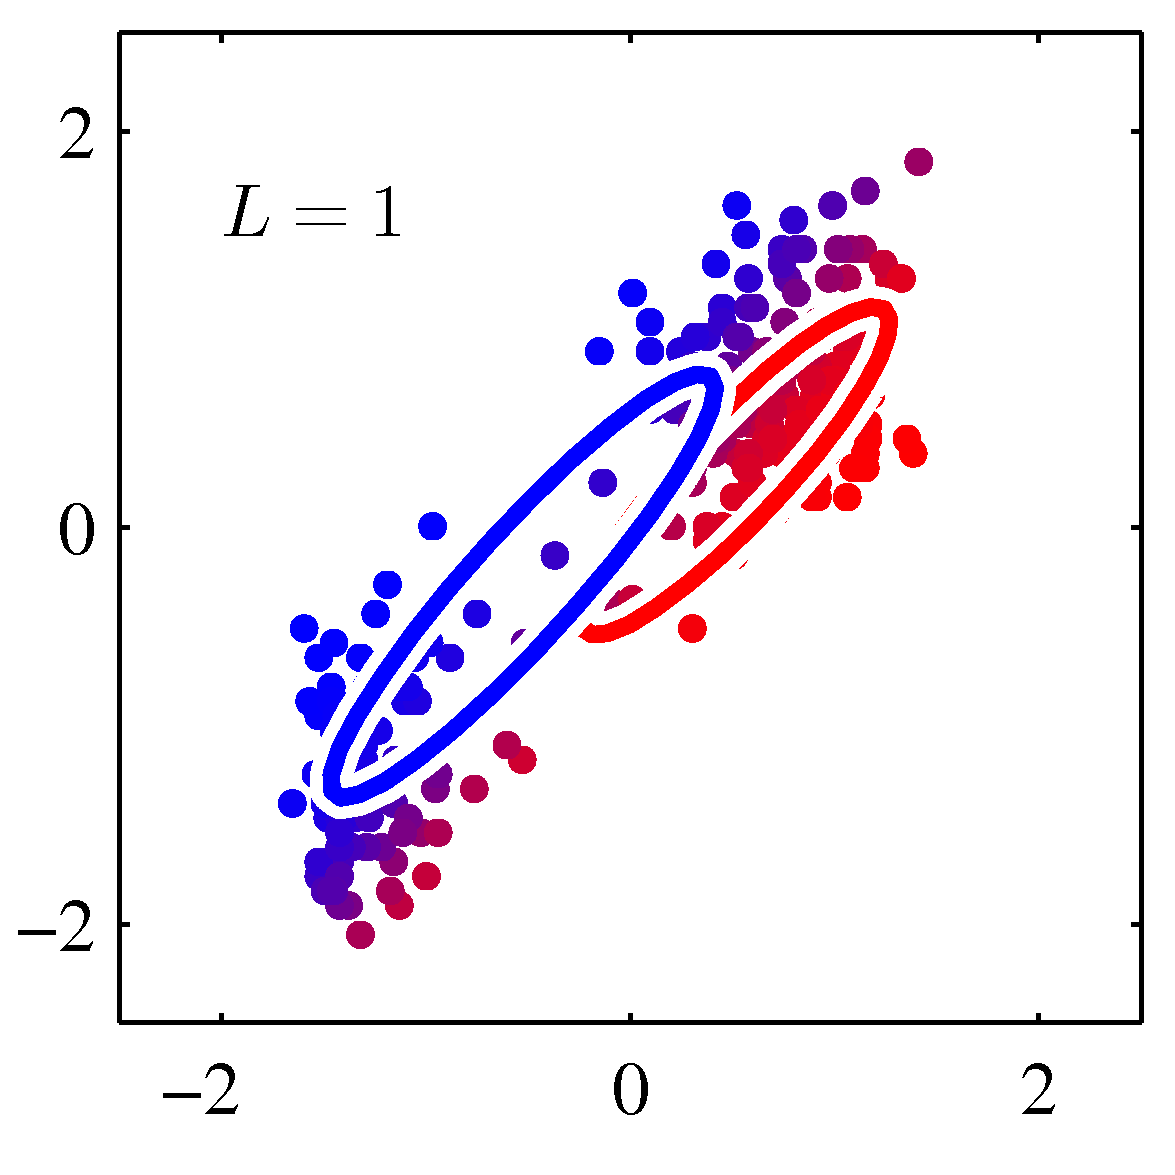
\includegraphics[width=0.25\textwidth]{GMM2}
\caption{Old Faithful data. GMM after one iteration of EM}
\label{fig:GMM2}
\end{figure}

\begin{figure}[H]
\centering
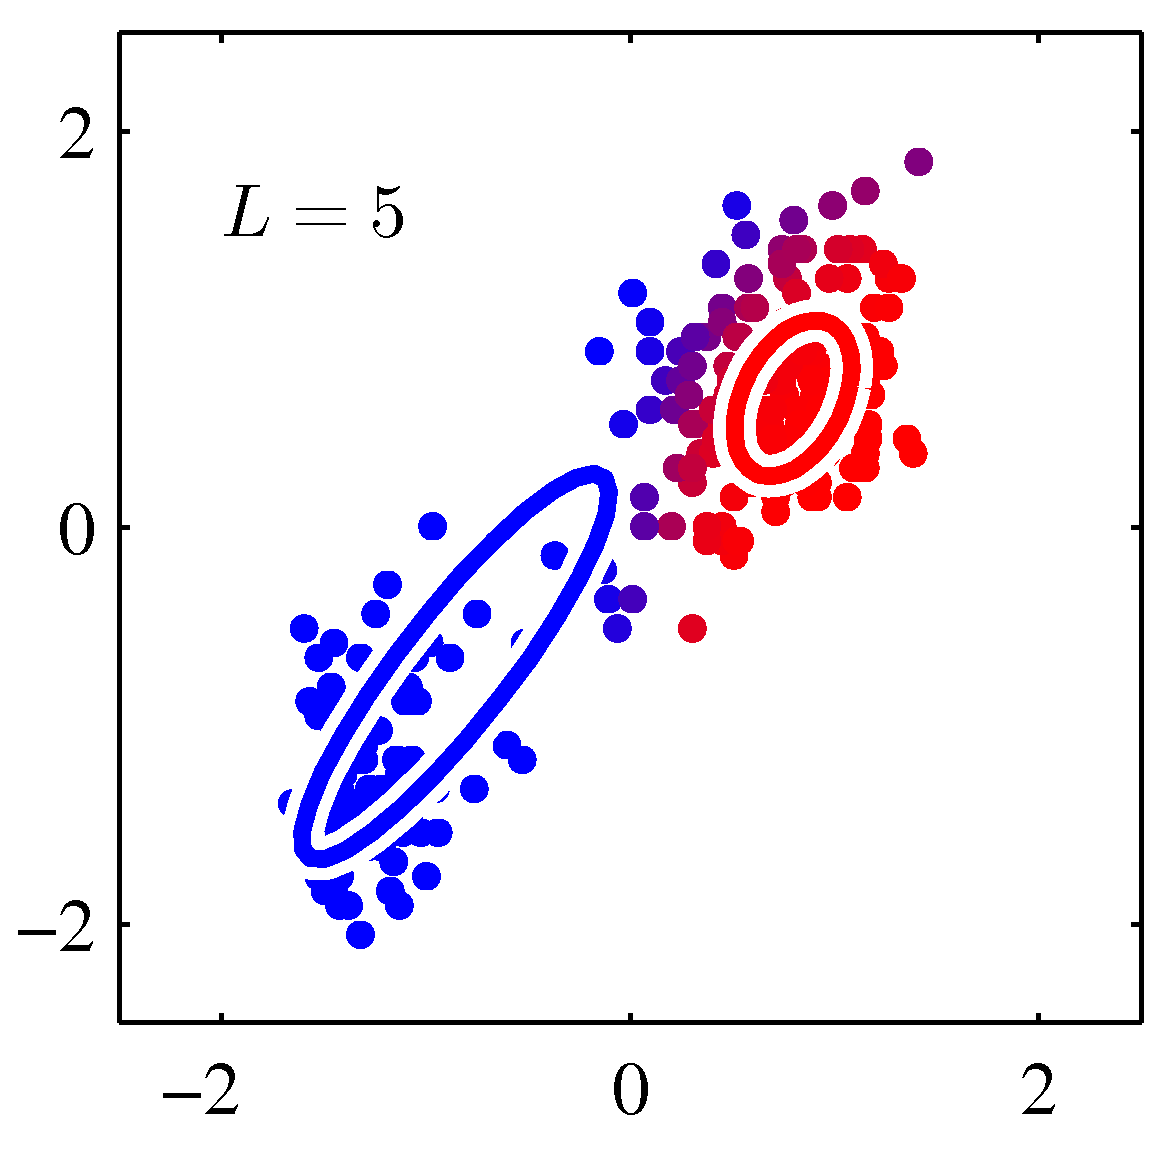
\includegraphics[width=0.25\textwidth]{GMM3}
\caption{Old Faithful data. GMM after five iterations of EM}
\label{fig:GMM3}
\end{figure}

After five iterations the EM has honed in on the centers of the two clusters (Figure \ref{fig:GMM3}).
Note that K-means could have reached roughly this point in as many iterations, but at much less computational cost.

\begin{figure}[H]
\centering
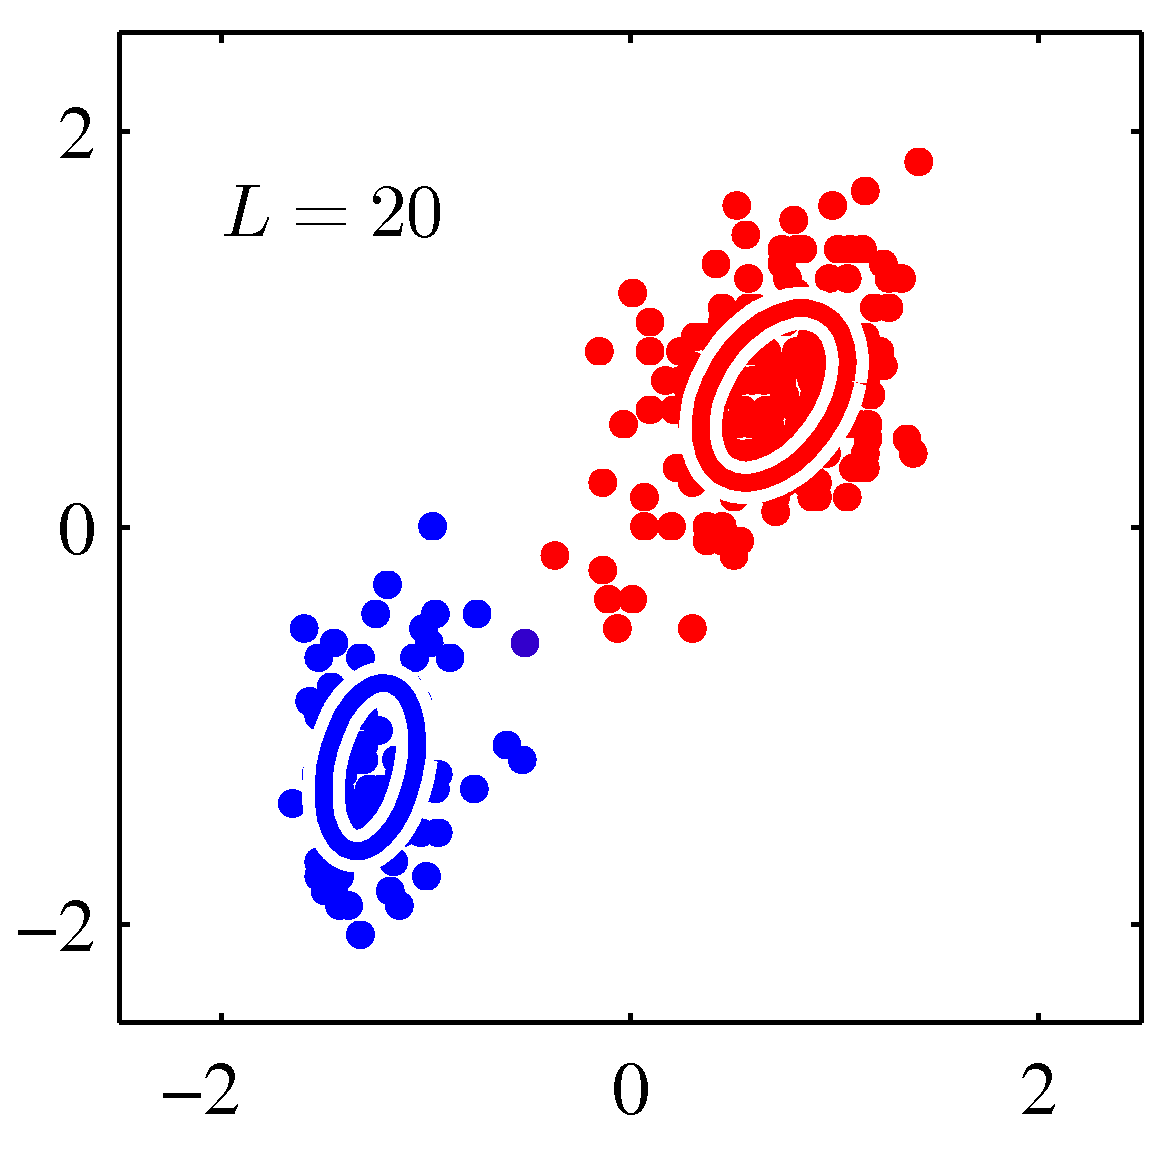
\includegraphics[width=0.25\textwidth]{GMM4}
\caption{Old Faithful data. GMM after 20 iterations of EM}
\label{fig:GMM4}
\end{figure}

As seen in Figure \ref{fig:GMM4} above the model has converged on a well-fitting model after 20 iterations.
This means that further iterations would be superfluous, as they would yield only negligible increases in overall likelihood of the GMM. \\

The specific procedure for estimating GMM parameters using EM is as follows \cite{bishop2007}: 

\subsection*{Initialization:}

Choose initial estimates for model parameters $ \mathbf{\pi}_{k}, \mathbf{\mu}_{k}, \mathbf{\Sigma}_{k} $.

\begin{itemize}

\item
$ k $ is the component number out of K.

\item
$ \pi_{k} $  is the weight of the \textit{k}th component.

\item
$ \mathbf{\mu}_{k}$ is the mean of the \textit{k}th component.

\item
$ \mathbf{\Sigma}_{k} $ is the covariance matrix of the \textit{k}th component.

\end{itemize}


Compute the initial log-likelihood og the model

\begin{equation} \label{eq:loglikeGMM}
\ln p\left(X | \mathbf{\mu}, \mathbf{\Sigma}, \pi\right) = 
\sum_{n=1}^{N} \ln \sum_{k=1}^{N} \pi_{k}\mathcal{N}(\mathbf{x}_{n}|\mathbf{\mu}_{k},\mathbf{\Sigma}_{k})
\end{equation}

\subsection*{E-step:}
Calculate the probability of each point in each component in order to assing responsibility

\begin{equation}
\gamma_{nk} = 
\frac
{\pi_{k}\mathcal{N}(\mathbf{x}_{n}|\mathbf{\mu}_{k},\mathbf{\Sigma}_{k})}
{\sum_{j=1}^{K} \pi_{n}\mathcal{N}(\mathbf{x}_{n}|\mu_{j},\mathbf{\Sigma}_{j})}
\end{equation}

\subsection*{M-step:}
Estimate new guesses for $ \mathbf{\pi}_{k}, \mathbf{\mu}_{k}, \mathbf{\Sigma}_{k} $.

\begin{equation}
\bm{\mu}_{k}^{new} = 
\frac{1}{N_{k}}
\sum_{n=1}^{N} 
\gamma_{nk}
\mathbf{x}_{k}
\end{equation}

\begin{equation}
\bm{\Sigma}_{k}^{new} = 
\frac{1}{N_{k}}
\sum_{n=1}^{N} 
\gamma_{nk}
(\mathbf{x}_{k} - \mathbf{\mu}_{k}^{new})
(\mathbf{x}_{k} - \mathbf{\mu}_{k}^{new})^{T}
\end{equation}

\begin{equation}
\pi_{k}^{new} =
\frac
{N_{k}}
{N}
\end{equation}

\subsection*{Convergence check:}

Recalculate log likelihood using Equation \ref{eq:loglikeGMM}.
If the log likelihood has not changed more than some predetermined threshold stop iteration.
Otherwise continue from E-step.



\section{Method}
The way GMM was applied in this project was, in simple, to generate a single GMM for each speaker using the training data.
Then the test set was classified by summing the log-likelihoods for each GMM for a number of sequential frames and then selecting the speaker with the highest sum of log-likelihoods.
This approach adds a measure of supervision to an otherwise unsupervised technique.
Further, because classification is done using a set of sequential frames, a temporal element is added.

\subsection{Training}
A GMM was trained for every speaker.
The feature data (both training and test data) has been subjected to PCA, in order to project the data onto a basis that aligned the variance along the dimensions without removing any dimensions. 
\fxnote{Prøv at fjerne et nogle dimensioner}
Then, for each speaker, a GMM is fitted to the respective speakers' training data, using MATLAB's Statistics Toolbox and the following parameters:

\begin{itemize}

\item
Number of components: \textit{8}

\item
Covariance matrix: \textit{Full}

\item
Initialization: \textit{Random}

\end{itemize}

\subsection{Classification}
Classification is done on the test data is done on super frames of 100 sequential frames.
The log-likelihood for each frame is summed over the entire super frame for each model.
\fxnote{Math that proves me right}
The model with the largest sum is chosen as winner.



\subsection{Results}
Using GMM has been tried with different data complexities.
Most notably, with speakers uttering the same single digit ("\textit{ZERO}"), two different digits ("\textit{ZERO}" and "\textit{ONE}"), and ten different digits ("\textit{ZERO}", "\textit{ONE}" through "\textit{NINE}").

\subsubsection{Single digit:}

\begin{figure}[H]
\centering
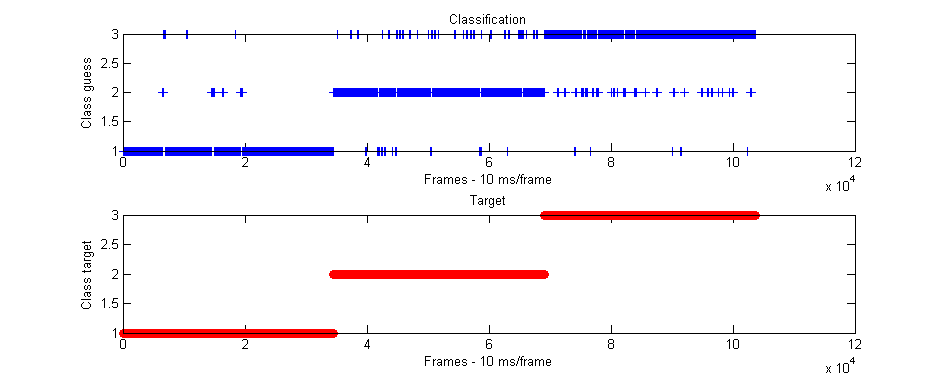
\includegraphics{GMM_10digit_8cent_3speak}
\caption{Results of using GMM with 3 speakers, 8 centers per model and 1 digit spoken}
\label{fig:GMM_fig_1}
\end{figure}

\begin{table}[H]                                                   
\centering                                                          
\begin{tabular}{|l|c|c|c|c|}                                        
\hline                                                              
  & Speaker Jacob & Speaker Mose & Speaker Simon & Precision [\%] \\
\hline                                                              
Estimate Jacob & 3400.0 & 0.0 & 0.0 & 100.0 \\                      
\hline                                                              
Estimate Mose & 54.0 & 2946.0 & 0.0 & 98.2 \\                       
\hline                                                              
Estimate Simon & 0.0 & 508.0 & 3454.0 & 87.2 \\                     
\hline                                                              
Sensitivity [\%] & 98.4 & 85.3 & 100.0 & 94.6 \\                    
\hline                                                              
\end{tabular}                                                       
\caption{Confusion matrix - 1 digit}                                
\label{table:GMM_conf_1}                                            
\end{table} 


\subsubsection{Two digits:}
\begin{figure}[H]
\centering
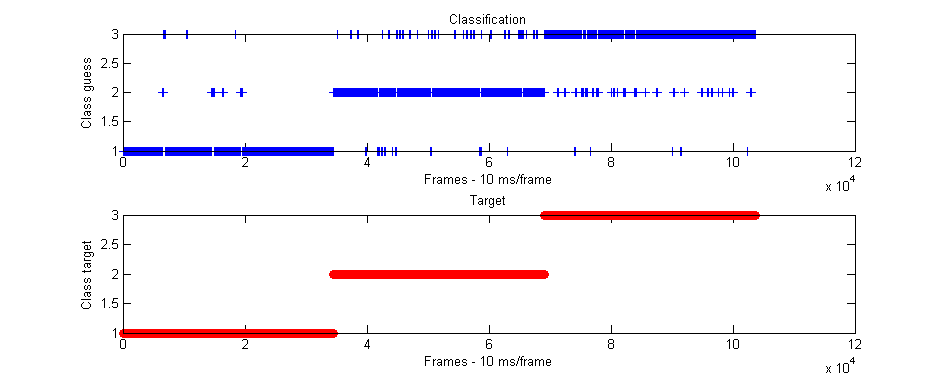
\includegraphics{GMM_10digit_8cent_3speak}
\caption{Results of using GMM with 3 speakers, 8 centers per model and 2 digits spoken}
\label{fig:GMM_fig_2}
\end{figure}

\begin{table}[H]                                              
\centering                                                     
\begin{tabular}{|l|c|c|c|c|}                                   
\hline                                                         
  & Speaker Jacob & Speaker Mose & Speaker Simon & Precision [\%] \\
\hline                                                         
Estimate Jacob & 6300.0 & 0.0 & 0.0 & 100.0 \\                 
\hline                                                         
Estimate Mose & 10.0 & 5790.0 & 100.0 & 98.1 \\                
\hline                                                         
Estimate Simon & 600.0 & 1120.0 & 6810.0 & 79.8 \\             
\hline                                                         
Sensitivity [\%] & 91.2 & 83.8 & 98.6 & 91.2 \\                
\hline                                                         
\end{tabular}                                                  
\caption{Confusion matrix - 2 digits}                          
\label{table:GMM_conf_2}                                       
\end{table} 
\subsubsection{Ten digits:}

\begin{figure}[H]
\centering
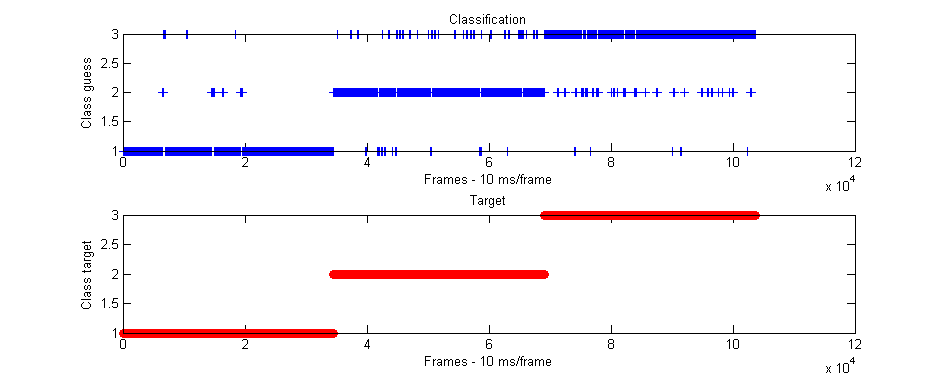
\includegraphics{GMM_10digit_8cent_3speak}
\caption{Results of using GMM with 3 speakers, 8 centers per model and 10 digits spoken}
\label{fig:GMM_fig_10}
\end{figure}

\begin{table}[H]                          
\centering                                                     
\begin{tabular}{|l|c|c|c|c|}                                   
\hline                                                         
  & Speaker Jacob & Speaker Mose & Speaker Simon & Precision [\%] \\
\hline                                                         
Estimate Jacob & 33000.0 & 1300.0 & 600.0 & 94.6 \\            
\hline                                                         
Estimate Mose & 1159.0 & 29341.0 & 3900.0 & 85.3 \\            
\hline                                                         
Estimate Simon & 400.0 & 3918.0 & 30059.0 & 87.4 \\            
\hline                                                         
Sensitivity [\%] & 95.5 & 84.9 & 87.0 & 89.1 \\                
\hline                                                         
\end{tabular}                                                  
\caption{Confusion matrix - 10 digits}                         
\label{table:GMM_conf_10}                                      
\end{table}

















